\documentclass[10pt, aspectratio=169]{beamer}

% Configurações de Idioma e Pacotes Matemáticos
\usepackage[brazilian]{babel}
\usepackage{amsmath,amssymb,amsthm}
\usepackage{graphicx}
\usepackage{booktabs}
\usepackage{tcolorbox}

% --- PALETA DE CORES INSTITUCIONAL ---
\definecolor{primary}{RGB}{10, 45, 90}       % Azul Escuro
\definecolor{secondary}{RGB}{25, 110, 180}   % Azul Destaque
\definecolor{bglight}{RGB}{245, 247, 250}    % Cinza Claro

% --- CONFIGURAÇÕES DO TEMA BEAMER ---
\usetheme{Boadilla}
\usecolortheme{default}

% Personalização de Cores dos Elementos Beamer
\setbeamercolor{structure}{fg=primary}
\setbeamercolor{palette primary}{bg=primary, fg=white}
\setbeamercolor{palette secondary}{bg=secondary, fg=white}
\setbeamercolor{palette tertiary}{bg=primary!80, fg=white}
\setbeamercolor{titlelike}{bg=primary, fg=white}
\setbeamercolor{frametitle}{bg=primary, fg=white}
\setbeamercolor{block title}{bg=secondary, fg=white}
\setbeamercolor{block body}{bg=bglight, fg=black}

% Remover botões de navegação no rodapé
\setbeamertemplate{navigation symbols}{}

% Rodapé Personalizado
\setbeamertemplate{footline}{
  \leavevmode%
  \hbox{%
  \begin{beamercolorbox}[wd=.333333\paperwidth,ht=2.25ex,dp=1ex,center]{author in head/foot}%
    \usebeamerfont{author in head/foot}Prof. Cleibson José da Silva
  \end{beamercolorbox}%
  \begin{beamercolorbox}[wd=.333333\paperwidth,ht=2.25ex,dp=1ex,center]{title in head/foot}%
    \usebeamerfont{title in head/foot}Matemática VI -- IFPE
  \end{beamercolorbox}%
  \begin{beamercolorbox}[wd=.333333\paperwidth,ht=2.25ex,dp=1ex,right]{date in head/foot}%
    \usebeamerfont{date in head/foot}\insertframenumber{} / \inserttotalframenumber\hspace*{2ex} 
  \end{beamercolorbox}}%
  \vskip0pt%
}

% --- DADOS DA APRESENTAÇÃO (Texto Puro nos Colchetes para o hyperref) ---
\title[Numeros Complexos]{Números Complexos: Forma trigonométrica}
\subtitle{Resolução de questões da lista 2}
\author[Prof. Cleibson]{Prof. Cleibson José da Silva}
\institute[IFPE]{
  Instituto Federal de Pernambuco -- Campus Caruaru \\
  \vspace{0.2cm}
  
\includegraphics[height=2cm]{Imagens/logocaruaru.png}
}
\date{}

\begin{document}

% --- SLIDE 1: TÍTULO ---
\begin{frame}
  \titlepage
\end{frame}

\begin{frame}[t]
 \textbf{Questão 7:} Determine as raízes quartas de $-16$.
\end{frame}

\begin{frame}[t]
 \textbf{Questão 9:} Entre os complexos $z$ tais que $|z+1+i|=1$, determine os de módulo máximo.
\end{frame}

\begin{frame}[t]
 \textbf{Questão 13:} (FUVEST-SP) Entre os números complexos $z = a + bi$, não nulos, que têm argumento igual a $\dfrac{\pi}{4}$, aquele cuja representação geométrica está sobre a parábola $y = x^2$ é:
  \begin{enumerate}[a)]
    \item $1 + i$
    \item $1 - i$
    \item $-1 + i$
    \item $\sqrt{2} + 2i$
    \item $-\sqrt{2} + 2i$
  \end{enumerate}

\end{frame}


\begin{frame}[t]

    \textbf{Questão 14:} (Cesgranrio) O conjunto dos pontos $z = x + yi$ do plano complexo que satisfazem $|z - 1|^2 = 2x$ e $y \ge 2$ é:
  
  \begin{enumerate}[a)]
    \item o conjunto vazio.
    \item uma região não limitada do plano.
    \item todos os pontos $x + yi$ tais que $y \ge 2$.
    \item uma reta.
    \item diferente dos quatro anteriores.
  \end{enumerate}

\end{frame}

 \begin{frame}[t]
 \textbf{Questão 16:} (UFU-MG) Sejam $z_1$ e $z_2$ dois números complexos representados geometricamente, na figura a seguir, pelos pontos $A$ e $B$ respectivamente.

  \begin{figure}[h!]
    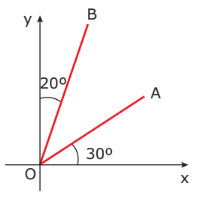
\includegraphics[scale=0.7]{Imagens/L2F3.png}
  \end{figure}

  Sabendo-se que $OA = 3\text{ cm}$ e que $OB = 6\text{ cm}$, pode-se afirmar que:
  \begin{enumerate}[a)]
    \item $\dfrac{z_2}{z_1}$ tem módulo igual a $2\text{ cm}$.
    \item $z_1 + z_2$ tem módulo igual a $9\text{ cm}$.
    \item O argumento de $z_2 - z_1$ é igual a $40^\circ$.
    \item O argumento de $z_2 \cdot z_1$ é igual a $50^\circ$.
  \end{enumerate}

 \end{frame}

\end{document}